\documentclass[11pt]{cernrep}
\usepackage{graphicx,epsfig}
\bibliographystyle{lesHouches}

\usepackage{xspace}
\newcommand{\Sherpa}{S\protect\scalebox{0.8}{HERPA}\xspace}
\newcommand{\Powheg}{P\protect\scalebox{0.8}{OWHEG}\xspace}
\newcommand{\CSS}{C\protect\scalebox{0.8}{SS}\xspace}
\newcommand{\Comix}{C\protect\scalebox{0.8}{OMIX}\xspace}
\newcommand{\Amegic}{A\protect\scalebox{0.8}{MEGIC++}\xspace}
\newcommand{\MCatNLO}{M\protect\scalebox{0.8}{C}@N\protect\scalebox{0.8}{LO}\xspace}
\newcommand{\MEPS}{M\scalebox{0.8}{E}P\scalebox{0.8}{S}\xspace}
\newcommand{\MEPSatNLO}{M\scalebox{0.8}{E}P\scalebox{0.8}{S}@N\protect\scalebox{0.8}{LO}\xspace}
\newcommand{\Collier}{C\protect\scalebox{0.8}{OLLIER}\xspace}
\newcommand{\OpenLoops}{O\protect\scalebox{0.8}{PEN}L\protect\scalebox{0.8}{OOPS}\xspace}
\newcommand{\Herwig}{H\protect\scalebox{0.8}{ERWIG}7\xspace}
\newcommand{\Matchbox}{M\protect\scalebox{0.8}{ATCHBOX}\xspace}
\newcommand{\MGaMC}{M\protect\scalebox{0.8}{AD}G\protect\scalebox{0.8}{RAPH}5\_aMC@NLO\xspace}
\newcommand{\MadGraph}{M\protect\scalebox{0.8}{AD}G\protect\scalebox{0.8}{RAPH}\xspace}
\newcommand{\MGAMC}{MG5\_aMC\xspace}
\newcommand{\MadGraphfour}{M\protect\scalebox{0.8}{AD}G\protect\scalebox{0.8}{RAPH}4\xspace}
\newcommand{\CVolver}{CV\protect\scalebox{0.8}{OLVER}\xspace}
\newcommand{\ColorFull}{C\protect\scalebox{0.8}{OLOR}F\protect\scalebox{0.8}{ULL}\xspace}
\newcommand{\MoCaNLO}{M\protect\scalebox{0.8}{oCaNLO}\xspace}
\newcommand{\Recola}{R\protect\scalebox{0.8}{ecola}\xspace}
\newcommand{\VBFNLO}{V\protect\scalebox{0.8}{BFNLO}\xspace}
\newcommand{\pt}{\ensuremath{p_{T}}\xspace}
\newcommand\sss{\mathchoice%
{\displaystyle}%
{\scriptstyle}%
{\scriptscriptstyle}%
{\scriptscriptstyle}%
}
\newcommand\MSB{\ifmmode {\overline{\rm MS}} \else $\overline{\rm MS}$\fi}
\newcommand\MINLO{{\tt MiNLO}}
\newcommand\muf{\mu_{\sss\rm F}}
\newcommand\mur{\mu_{\sss\rm R}}
\newcommand\KRA{K_{\scriptscriptstyle \rm R}}
\newcommand\KFA{K_{\scriptscriptstyle \rm F}}

\newcommand{\GOSAM}{G\protect\scalebox{0.8}{O}S\protect\scalebox{0.8}{AM}\xspace}
\newcommand{\POWHEGBOX}{P\protect\scalebox{0.8}{OWHEG} B\protect\scalebox{0.8}{OX}\xspace}
\newcommand{\QGRAF}{Q\protect\scalebox{0.8}{GRAF}\xspace}
\newcommand{\FORM}{F\protect\scalebox{0.8}{ORM}\xspace}
\newcommand{\SAMURAI}{S\protect\scalebox{0.8}{AMURAI}\xspace}
\newcommand{\GOLEM}{G\protect\scalebox{0.8}{OLEM}\xspace}
\newcommand{\NINJA}{N\protect\scalebox{0.8}{INJA}\xspace}
\newcommand{\SPINNEY}{S\protect\scalebox{0.8}{PINNEY}\xspace}
\newcommand{\ONELOOP}{O\protect\scalebox{0.8}{NE}LO\protect\scalebox{0.8}{OP}\xspace}
\newcommand{\MCFM}{M\protect\scalebox{0.8}{CFM}\xspace}

% Commands defined by Mathieu
\usepackage{amsmath}
\newcommand{\MP}[1]{{ {\color{blue}{ [MP: #1]}} }}
\newcommand{\KL}[1]{{ {\color{yellow}{ [KL: #1]}} }}
\newcommand{\SB}[1]{{ {\color{green}{ [SB: #1]}} }}

\usepackage{color}
\usepackage{morefloats}

\begin{document}

\section{Study of electroweak production of WZ in association with two jets at the LHC 
\protect\footnote{Section coordinators: K.~Long, M.~Pellen}$^{,}$ 
\protect\footnote{Contributing authors: S.~Br\"auer, V.~Ciulli, S.~Gieseke, M.~Herndon, M.~Mozer, S.~Pl{\"a}tzer, M.~Rauch, E.~Yazgan.}$^{,}$
\protect\footnote{The work of SB is supported by German Federal Ministry for Education and Research (BMBF) under contract 05H15MGCAA.
MP acknowledges financial support by the BMBF under contract no.~05H15WWCA1 and the German Science Foundation (DFG) under reference number DE 623/6-1 .
\MP{Missing acknowledgements. Please do it.}
\label{vbs_section}}}

\subsection{Introduction \label{vbs_intro}}

The electroweak (EW) production of vector-boson pairs in association with two jets at the CERN Large Hadron Collider (LHC) forms an important class of processes both theoretically and experimentally.
This signature includes vector-boson scattering (VBS) contributions, which constitute the principle example of processes where the scattering of two massive gauge bosons can be observed at the LHC.
These processes provide a natural probe of the vector boson quartic couplings, which arise due to the non-Abelian nature of the electroweak gauge group and are exactly predicted by the SM.
The Higgs boson plays a unique role in these interactions, preventing the cross section from diverging in the high-energy limit and preserving the unitarity of the associated scattering amplitudes.
Deviations in these channels could therefore indicate physics in the electroweak sector beyond the standard model.

Measurements of these processes are particularly challenging due to the high multiplicity of the processes and their small cross sections, and 
have only been observed and even measured recently by the experimental collaborations at the LHC.
The most precise current measurement \cite{Aad:2014zda,Khachatryan:2014sta,Sirunyan:2017ret,Aaboud:2016ffv} concerns the scattering of two same sign W bosons (usually denoted ${\rm W}^\pm{\rm W}^\pm{\rm j}{\rm j}$).
This process has a unique signature due to the same-sign charged leptons in the final state.
The cross section is well within reach with the large datasets being collected in the LHC Run II, and the
signature is experimentally accessible due to the precise lepton identification, charge, and momentum resolution of the LHC experiments.
The nature of the final state is also attractive due to the low rate of background processes
producing two prompt, same sign leptons associated with forward jets (referred to as the irreducible background).

Measurements of other VBS signatures such as ${\rm Z}{\rm Z}{\rm j}{\rm j}$, ${\rm W}^+{\rm W}^-{\rm j}{\rm j}$, or ${\rm W}^{\pm}{\rm Z}{\rm j}{\rm j}$ present additional challenges due to the lower cross section and larger irreducible backgrounds, which dominate over the VBS contribution in most regions of phase space.
Nonetheless, observations have already been performed at the LHC for both the ${\rm Z}{\rm Z}{\rm j}{\rm j}$ \cite{Sirunyan:2017fvv} and ${\rm W}^{\pm}{\rm Z}{\rm j}{\rm j}$ \cite{Aad:2016ett} scattering at $\sqrt{s} = 8$~TeV.
In these cases, separation of the electroweak component of the VVjj state relies on exploiting the different characteristics of the VBS and non-VBS
components through kinematic selections, which relies on theoretical predictions.
Accurate predictions and a detailed understanding of their associated uncertainties therefore directly impact such measurements.
A theory-agnostic measurement that does not attempt separation of states by production mode avoids such dependencies,
but cannot fully leverage the statistical tools and treatment of uncertainties available in an experimental analysis.
The approaches are therefore complementary, and are often presented together in experimental results.

From a theoretical point of view, one of the challenges for the predictions of the EW di-boson production in association with two jets is its high multiplicity.
This explains why in the past, next-to-leading order (NLO) predictions have focused on VBS approximations.
Only recently, full NLO computations became available at NLO QCD and EW for both the EW component and the QCD-induced process for ${\rm W}^\pm{\rm W}^\pm{\rm j}{\rm j}$ \cite{Biedermann:2017bss}.
For this process, preliminary results \cite{Anders:2018gfr} of a comparison of different theoretical predictions have shown that differences between the full computation and VBS-approximated ones are not significant given the present experimental accuracy.
Qualitatively, one could expect a similar conclusion for other processes such as ${\rm W}^{\pm}{\rm Z}{\rm j}{\rm j}$ but an explicit check is still worth doing.
Therefore, in this proceedings we aim at making a similar comparison of theoretical predictions implemented in Monte Carlo programs.
This allows to infer the quality of the VBS approximation at leading-order (LO).

As such there is strong motivation for an investigation of the theoretical tools, predictions, and uncertainties
used in a typical VBS analysis. 
We focus on the ${\rm W}^{\pm}{\rm Z}{\rm j}{\rm j}$ \cite{Aad:2016ett} state, the measurement of which was strongly limited by the size of the dataset, 
but which has not yet been studied at the 13 TeV LHC. Hence, a preliminary study on this process is of particular interest.

Due to its colour structure, the ${\rm W}^{\pm}{\rm Z}{\rm j}{\rm j}$ signature possesses three different contributions at LO.
The first, of order $\mathcal{O} (\alpha^6)$, is usually referred to as the EW component or even VBS component (even if it also possesses non-VBS contributions such as tri-boson ones).
The two quark lines can also be connected via a gluon while the gauge bosons are radiated off the quark lines.
This contribution is of order $\mathcal{O} (\alpha_{\rm s}^2\alpha^4)$ and is called QCD contribution/background.
Finally, due to its structure, there exists a non-zero interference of order $\mathcal{O} (\alpha_{\rm s}\alpha^5)$.
For this signature (as opposed to \emph{e.g.}\ ${\rm W}^\pm{\rm W}^\pm{\rm j}{\rm j}$) the EW component is very suppressed with respect to the QCD one.
This implies having very exclusive experimental cuts in order to enhance the EW contribution and a good control over the description of both the EW signal and QCD background.
To that end, the understanding of theoretical predictions and Monte Carlo programs is key.
In particular, it is vital to ensure that all different programs can provide equivalent physics result.
Such comparisons can also shed light on the true uncertainties of such predictions.
In addition to the typical uncertainty treatments asses the impact of parton density function (PDF) 
uncertainties or of missing higher orders in perturbative QCD, Monte Carlo generators require many input parameters,
the selection of which  can have a significant impact on the predictions both in shape and normalisation.
In the present study we use a common set-up for all predictions at LO accuracy. We additionally provide results with
variations in some parameters and comment on their effects and motivations.

In these proceedings, we start with Sec.~\ref{vbs_theory} where a short review of the theoretical state-of-the-art predictions is given.
The programs used in the present work are also briefly described.
In Sec.~\ref{setup}, the set-up of the calculation is presented.
It amounts to give the input parameters as well as the event selection.
Section~\ref{vbs_results} is devoted to the results of the study.
It starts with LO predictions for the three different contributions to the ${\rm e}^+  \nu_{\rm e}  \mu^+ \mu^- {\rm j} {\rm j}$ final state at the LHC.
Then the various comparisons are reported at both fixed order and with parton shower.
Finally, Sec.~\ref{vbs_concl} contains a summary, concluding remarks as well as recommendations.

\subsection{Theory and event generators \label{vbs_theory}}

The study focuses on the ${\rm W}^{\pm}{\rm Z}{\rm j}{\rm j}$ signature and more precisely on the partonic processes

\begin{equation}
 {\rm p} {\rm p} \to {\rm e}^+  \nu_{\rm e}  \mu^+ \mu^- {\rm j} {\rm j} ,
\end{equation}
%
and
%
\begin{equation}
 {\rm p} {\rm p} \to {\rm e}^-  \bar \nu_{\rm e}  \mu^+ \mu^- {\rm j} {\rm j}.
\end{equation}
%
The predictions presented are all at LO but NLO QCD corrections to the EW contribution and its irreducible background are already known.
The QCD corrections to the EW contributions are known since 10 years in the VBS approximation \cite{Bozzi:2007ur} while the QCD corrections to the QCD-induced process have been computed more recently \cite{Campanario:2013qba}.
The NLO EW corrections are currently unknown.
In Ref.~\cite{Biedermann:2016yds}, it has been argued that large NLO EW corrections to the EW contributions are an intrinsic feature of VBS at the LHC.
Therefore, they are expected to play a significant role for all VBS signatures.
In Ref.~\cite{Biedermann:2017bss}, which focuses on the computation of the full NLO corrections to the ${\rm W}^\pm{\rm W}^\pm{\rm j}{\rm j}$ process, it has been shown that the EW corrections to the EW process are the dominant NLO corrections.
This means that the EW corrections to the EW contributions are expected to be at least of the same order than the QCD ones for other VBS signatures.
\MP{Add some comments/references on parton shower to be added by Michael/Simon.}

In the following, the codes used for the predictions are briefly described.

\subsubsection*{\protect\MGaMC \label{vbs_mgamc}}

{\sc MadGraph5\_aMC@NLO}~\cite{Alwall:2014hca} is an automatic meta-code (a code that generates codes) which makes it possible to simulate any scattering process
      including NLO QCD corrections both at fixed order and including matching to parton showers. 
      The commands that have been used for the present computation are
      \MP{To be finalised by Kenneth}
\begin{verbatim}
> set complex_mass_scheme #1
> generate XXX #2
> output #3
\end{verbatim}
  The version used is .
  
\subsubsection*{\protect\Herwig \label{vbs_herwig}}

Based on extensions of the previously developed \Matchbox
module~\cite{Platzer:2011bc}, the \Herwig event generator~\cite{Bellm:2015jjp,Bahr:2008pv} facilitates the automated set-up of all ingredients necessary for a full NLO QCD calculation.
It relies on an implementation of the Catani--Seymour dipole
subtraction method~\cite{Catani:1996vz,Catani:2002hc}, as well as
interfaces to a list of external matrix element providers -- either
at the level of squared matrix elements, based on extensions of the
BLHA standard~\cite{Binoth:2010xt,Alioli:2013nda,Andersen:2014efa} or
at the level of colour-ordered sub-amplitudes.

For this study the relevant tree-level matrix elements have been
provided by an interface to VBFNLO \cite{Arnold:2008rz,Arnold:2011wj,Baglio:2014uba} using an extension of the BLHA
accord. We have matched these calculations to the angular ordered
shower using the subtractive matching and default settings of the
\Herwig~7.1 release. The PDF sets that have been used to tune the parton shower are MMHT2014lo68cl and
MMHT2014nlo68cl~\cite{Harland-Lang:2014zoa} ones.
These sets are not the one used for this computation (see below).
This can in particular impact initial-state radiations.
We consider variations of the hard shower scale as detailed in Ref.~\cite{Bellm:2016rhh}, using the 'resummation' profile scale choice.

\subsubsection*{\protect{\MoCaNLO\!+\Recola} \label{vbs_MoCaNLO_Recola}}

The program {\sc MoCaNLO+Recola} is made of a flexible Monte Carlo program dubbed {\sc MoCaNLO} and of the general matrix element generator {\sc Recola}~\cite{Actis:2012qn,Actis:2016mpe}.
The program can compute arbitrary processes in the Standard Model with NLO QCD and EW accuracy.
The fast integration is ensured by using similar phase-space mappings to those of Refs.~\cite{Berends:1994pv,Denner:1999gp,Dittmaier:2002ap}.
The complex-mass scheme~\cite{Denner:1999gp,Denner:2005fg} to treat unstable particles is always used.
These tools have been successfully used for the computation of NLO corrections for high-multiplicity processes and in particular VBS processes \cite{Biedermann:2016yds,Biedermann:2017bss}.

\subsubsection*{\protect\Sherpa \label{vbs_sherpa}}
\Sherpa~\cite{Gleisberg:2008ta,Gleisberg:2003xi} is a multipurpose event generator for high-energy particle collisions. 
It is built out of several algorithms and modules tailored to many different physics challenges of collider physics.
In the \Sherpa framework the infrared divergences appearing in the real-emission are treated by the Catani--Seymour dipole-subtraction method~\cite{Catani:1996vz,Catani:2002hc,Gleisberg:2007md}. 
The default parton-shower algorithm of \Sherpa is based on the Catani--Seymour factorisation~\cite{Schumann:2007mg,Hoeche:2009xc}.
For NLO computations, interfaces to several one-loop generators exist, with the interface to \textsc{Recola}~\cite{Actis:2012qn,Actis:2016mpe} being the latest addition~\cite{Biedermann:2017yoi}.
For correctly combining the matrix elements in multijet-production processes with the parton shower, \Sherpa has adapted the MEPS@LO method~\cite{Hoeche:2009rj} at LO and its generalisation MEPS@NLO~\cite{Hoche:2010kg} at NLO. 
In this study, the matrix elements are provided by \textsc{Comix}~\cite{Gleisberg:2008fv}, one of the two built-in generators next to \textsc{Amegic}~\cite{Krauss:2001iv}.
Both of the studied partonic processes are then showered with the default shower.

\subsubsection*{\protect\VBFNLO \label{vbs_VBFNLO}}
\VBFNLO~\cite{Arnold:2008rz,Arnold:2011wj,Baglio:2014uba} is a flexible
Monte-Carlo event generator for processes with electroweak bosons.
Besides the Standard Model, selected processes can also be calculated in
a variety of new-physics models, including effective field theories with
dimension-6 and dimension-8 operators.
Its use of leptonic tensors in the calculation of the matrix elements
can lead to a significant speed improvement compared to automatically
generated code.
For results with parton showers in this study, \VBFNLO serves as the
matrix-element provider and phase-space generator for \Herwig. The
interface between the two programs is based on an extension of the BLHA
standard~\cite{Binoth:2010xt,Alioli:2013nda,Andersen:2014efa}.
\MP{@Michael: Some comments on the matrix elements? Not full matrix element?}


\subsection{Details of the set-up \label{setup}}

In this section we describe default input parameters that have been used.
Also, the event selection used in the comparison are described.

\subsubsection*{Input parameters}

All simulations are performed for the LHC running with a center-of-mass energy $\sqrt s = 13 {\rm~TeV}$.
The default PDF used is the NNPDF~3.0 set~\cite{Ball:2014uwa} with four active flavour at LO and a strong coupling constant $\alpha_{\rm s}\left( M_{\rm Z} \right) = 0.130$.\footnote{Its {\tt lhaid} in LHAPDF6~\cite{Buckley:2014ana} is 263400.} 
% NNPDF30_lo_as_0130_nf_4 
If this default PDF is not employed, it is explicitly stated.
%
The masses and widths of the particle used in the simulations are
%
\begin{alignat}{2}
                M_{\rm t}   &=  173.21 {\rm~GeV},             & \quad \quad \quad \Gamma_{\rm t} &= 0 {\rm~GeV},  \nonumber \\
                M_{\rm Z}^{\rm OS} &=  91.1876{\rm~GeV},      & \quad \quad \quad \Gamma^{\rm OS}_{\rm Z} &= 2.4952{\rm~GeV},  \nonumber \\
                M_{\rm W}^{\rm OS} &=  80.385{\rm~GeV},       & \Gamma^{\rm OS}_{\rm Z} &= 2.085{\rm~GeV},  \nonumber \\
                M_{\rm H} &=  125.0{\rm~GeV}, 		      & \Gamma_{\rm H}   &=  4.07 \times 10^{-3}{\rm~GeV}.
\end{alignat}
%
The value of the mass and width of the Higgs boson are the ones recommended by the Higgs cross section working group \cite{deFlorian:2016spz}.
The top quark does not appear at tree level in the simulations when the bottom-quarks in the initial state are neglected.
Therefore its width is set to zero.
The numerical values used in the simulation for the pole mass/width of the gauge bosons ($V={\rm W,Z}$) are obtained from the measured on-shell (OS) values for the masses and widths according to Ref.~\cite{Bardin:1988xt} as:
%
\begin{equation}
        M_V = M_{\rm V}^{\rm OS}/\sqrt{1+(\Gamma_{\rm V}^{\rm OS}/M_{\rm V}^{\rm OS})^2}\,,\qquad  \Gamma_V = \Gamma_{\rm V}^{\rm OS}/\sqrt{1+(\Gamma_{\rm V}^{\rm OS}/M_{\rm V}^{\rm OS})^2}.
\end{equation}
%
The EW coupling is renormalised in the $G_\mu$ scheme \cite{Denner:2000bj} where
%
\begin{equation}
    G_{\mu}    = 1.16637\times 10^{-5}{\rm~GeV}^{-2}.
\end{equation}
%
With the previous input parameters, it corresponds to a numerical value for $\alpha$ of
%
\begin{equation}
 \alpha = 7.555310522369 \times 10^{-3}.
\end{equation}
%
Note that for the EW contribution of order $\mathcal{O} (\alpha^6)$, no dependence on the strong coupling appears.
For contributions (interference or QCD-induced contributions) where there is a dependence on $\alpha_{\rm s}$, the numerical value used is the one (potentially dynamically) extracted from the PDF set.

For the renormalisation and factorisation scales, two choices have been adopted.
For the fixed scale, it is
%
\begin{equation}
 \mu = \mu_{\rm fix} = M_{\rm W},
\end{equation}
%
while the dynamical scale used is
%
\begin{equation}
 \mu = \mu_{\rm dyn} = {\rm Max}\left[p_{\rm T, j}\right].
\end{equation}
%
The latter should be understood as the maximum of the transverse momenta of the tagging jets (defined below).
\MP{Justification for this scale choice? For Michael/Simon}
These two scale are the default fixed and dynamical scale, respectively.
If the scale used are different, this is explicitly stated in the text.

Photon-induced as well as bottom-induced contributions have been neglected.
The photon contributions are expected to be small \cite{Biedermann:2017bss} while the bottom-induced contribution can lead to single-top resonant contributions.
The later can in principle be isolated thanks to kinematical constraints.

\subsubsection*{Event selection}

Following experimental studies \cite{Aad:2016ett,CMS-PAS-SMP-14-008}, the event selection used for the present work is:

\begin{itemize}
\item All charged leptons are required to have
    \begin{align}
        \label{cut:1}
         p_{\rm T, \ell} >  20{\rm~GeV},\qquad |y_{\ell}| < 2.5.
    \end{align}
\item For the leptons of opposite charge and same flavour, an invariant mass cut to single out the Z-boson resonance is applied:
    \begin{align}
        \label{cut:2}
         76 {\rm~GeV} < m_{l_i^+ l_i^-} < 106 {\rm~GeV}.
    \end{align}

\item QCD jets are clustered thanks to the anti-$k_T$ algorithm~\cite{Cacciari:2008gp} with radius parameter $R=0.4$.
      At least two jets are required to have
        \begin{align}
        \label{cut:3}
         p_{\rm T, j} >  30{\rm~GeV}, \qquad |y_{\rm j}| < 4.7, \qquad \Delta R_{\rm j \ell} > 0.4,
        \end{align}
        %
        and are called tagging jets.
\item On the two leading tagging jets, typical VBS cuts are applied:
        \begin{align}
        \label{cut:4}
         m_{\rm j j} >  500{\rm~GeV},\qquad |\Delta y_{\rm j j}| > 2.5.
        \end{align}
\end{itemize}

These cuts have been issued either directly in the Monte Carlo programs or using a {\sc Rivet} routine \cite{Buckley:2010ar}.
This file will be made public in order to make the present study easily reproducible.

\subsection{Results \label{vbs_results}}

\subsubsection*{Several contributions for one process}

As explained previously, the processes ${\rm p} {\rm p} \to {\rm e}^+  \nu_{\rm e}  \mu^+ \mu^- {\rm j} {\rm j}$  and ${\rm p} {\rm p} \to {\rm e}^-  \bar \nu_{\rm e}  \mu^+ \mu^- {\rm j} {\rm j}$
possess at LO three contributions of orders $\mathcal{O} (\alpha^6)$, $\mathcal{O} (\alpha_{\rm s}\alpha^5)$, and $\mathcal{O} (\alpha_{\rm s}^2\alpha^4)$.
As it can be seen in Table~\ref{table:xsectallLOdyn}, the EW component represents only about $20\%$ of the total cross section.
This is in contrast with the ${\rm W}^\pm{\rm W}^\pm{\rm j}{\rm j}$ signature where the EW component represents almost $90\%$ of the cross section \cite{Biedermann:2017bss} in a comparable fiducial volume.
Hence measuring the EW component is much more challenging.
Therefore, inferring the shape of the signal and irreducible background is key.
Note that the interference contribution is about $0.5\%$ which is negligible with respect to current experimental accuracy.\footnote{For the ${\rm W}^\pm{\rm W}^\pm{\rm j}{\rm j}$ signature, the interference contribution has been shown to be around $3\%$ \cite{Biedermann:2017bss}.}

\begin{table}
\begin{center} 
\begin{tabular}{ c | c | c }
 $\mu = \mu_{\rm dyn}$ / $\sigma_{\rm LO}$ [fb] & ${\rm p} {\rm p} \to {\rm e}^+  \nu_{\rm e}  \mu^+ \mu^- {\rm j} {\rm j}$  & ${\rm p} {\rm p} \to {\rm e}^-  \bar \nu_{\rm e}  \mu^+ \mu^- {\rm j} {\rm j}$  \\
  \hline\hline
  $\mathcal{O} (\alpha^6)$                        & $0.25416(6)$  & $0.15003(3)$   \\
  $\mathcal{O} (\alpha_{\rm s}\alpha^5)$          & $0.006833(6)$ & $0.003977(3)$  \\
  $\mathcal{O} (\alpha_{\rm s}^2\alpha^4)$        & $0.9912(2)$   & $0.6306(6)$   \\
  \hline
\end{tabular}
\end{center}
\caption{
Fiducial cross sections at LO for the process ${\rm p}{\rm p}\to{\rm e}^+\nu_{\rm e}\mu^+\mu^-{\rm j}{\rm j}$ and ${\rm p}{\rm p}\to{\rm e}^-\bar\nu_{\rm e}\mu^+\mu^-{\rm j}{\rm j}$ at orders $\mathcal{O} (\alpha^6)$, $\mathcal{O} (\alpha_{\rm s}\alpha^5)$, and $\mathcal{O} (\alpha_{\rm s}^2\alpha^4)$.
The predictions are expressed in fb and are for the LHC running at a centre-of-mass energy of $\sqrt{s}=13 {\rm~TeV}$.
The scale used in the simulations is $\mu = \mu_{\rm dyn} = {\rm Max}\left[p_{\rm T, j}\right]$.
The integration errors of the last digits are given in parentheses.}
\label{table:xsectallLOdyn}
\end{table}

In Fig.~\ref{fig:diffcontr}, several differential distributions are shown.
In the upper plot the absolute predictions for each component as well as their sum are displayed.
In the lower plot, each contribution is normalised to their sum and expressed in per cent.
These distributions reflect the same conclusion as for the cross section namely that the processes are largely dominated by QCD-induced contribution.
The first two observables displayed (top) are the invariant mass and the rapidity difference of the two tagging jets.
These two observables are used as cuts [see Eq.~\eqref{cut:4}] in order to enhance the EW component over the QCD background.
The cuts are clearly visible on the plots and it is easily understandable why they are enhancing the EW contribution.
Toward high invariant-mass, the EW component becomes more and more important.
It even becomes of the same size as the QCD one for an invariant-mass of $2000{\rm~GeV}$.
The same holds true for high rapidity separation for the two jets.
On the other hand, the transverse invariant mass (bottom left) of muon--anti-muon pair does not display significant differences in the different contributions over the whole range.
Other transverse-momentum distributions displays the same pattern.
Finally, we show the distance between the two jets.
This observable also seems to possess a good discriminating power.
In particular, for large distances, the EW component becomes dominant but with very low statistics.
Concerning the interferences, they are extremely suppressed inheriting the cross section normalisation.
In none of the studied observables, their contribution exceed the per-cent level over the whole phase-space range.

\begin{figure}[htbp]
\begin{center}
   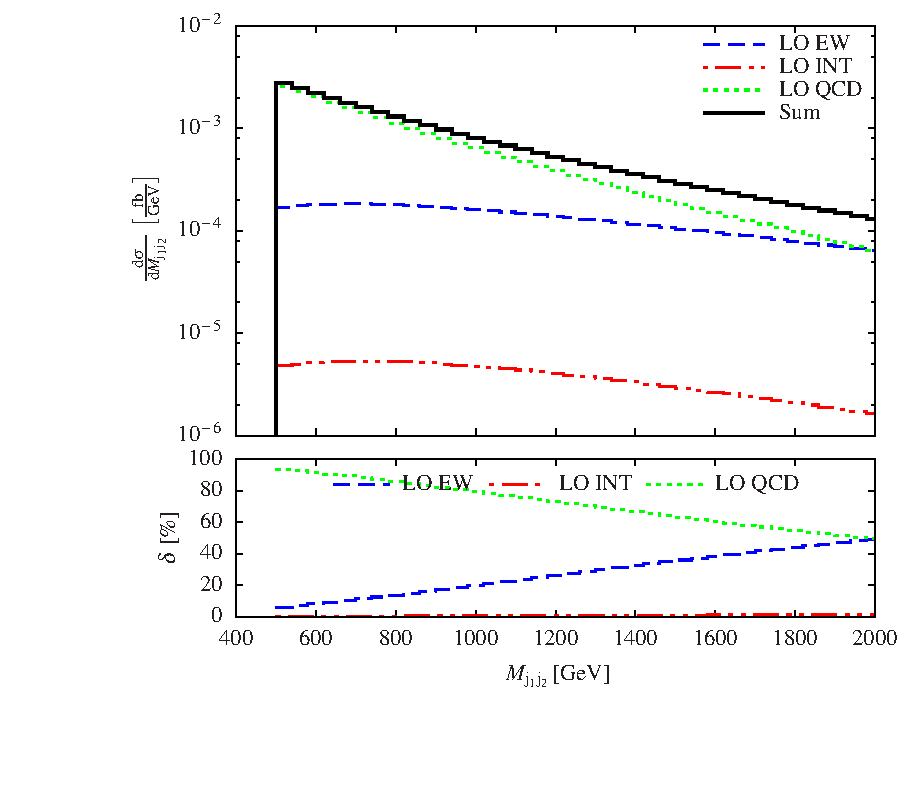
\includegraphics[scale=0.5]{figs/histogram_invariant_mass_mjj12}
   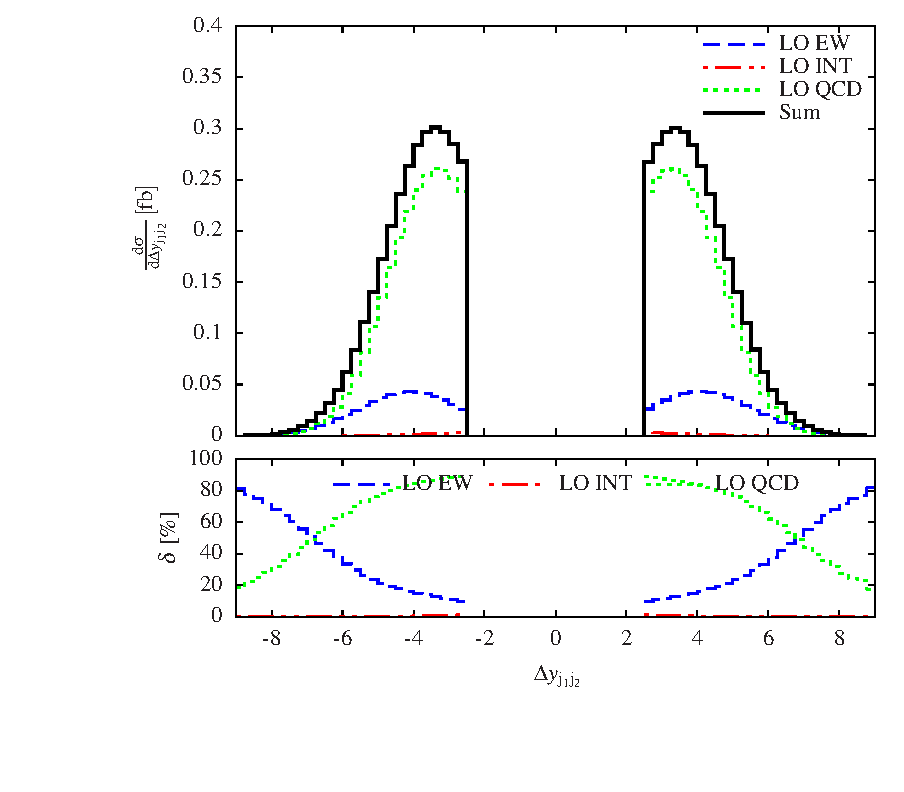
\includegraphics[scale=0.5]{figs/histogram_rapidity_separation_j1j2}
   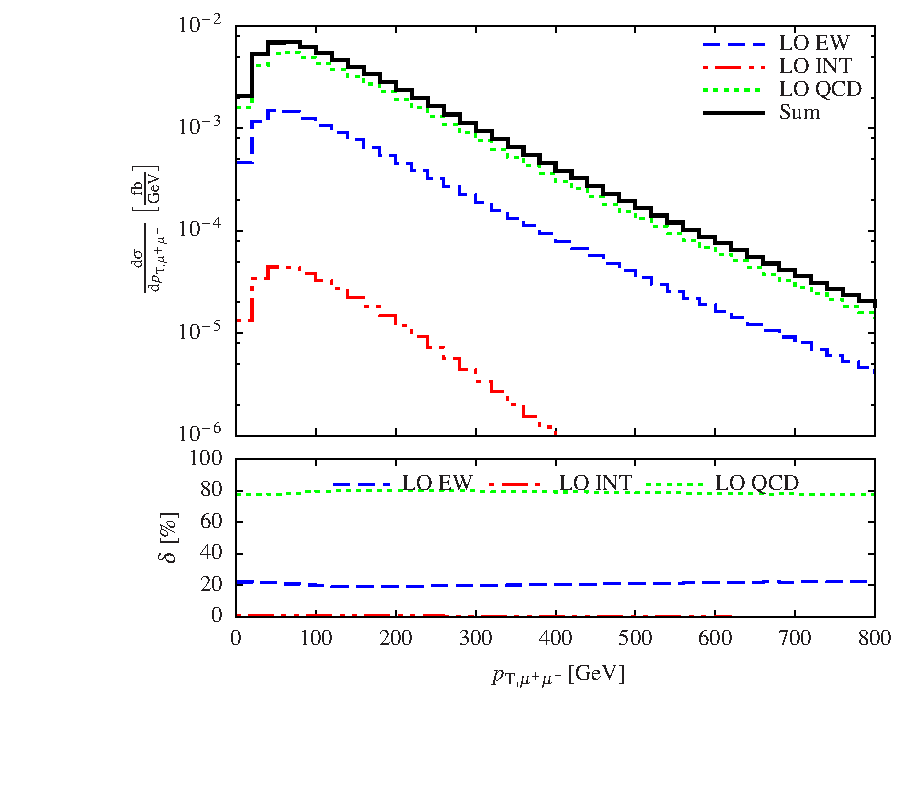
\includegraphics[scale=0.5]{figs/histogram_transverse_momentum_muamu}
   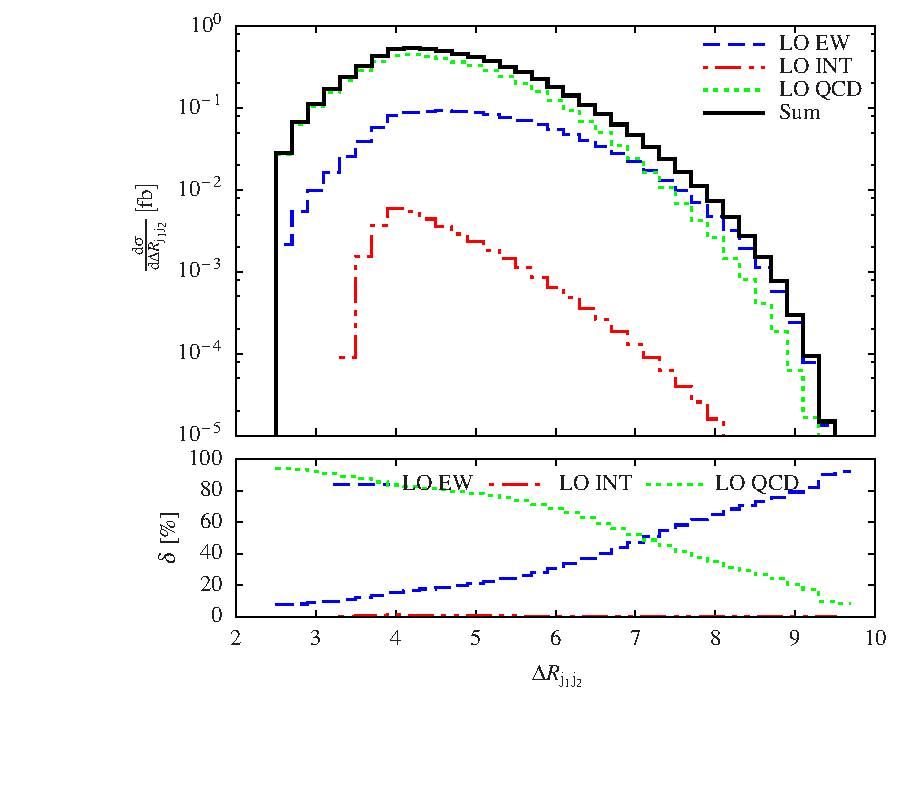
\includegraphics[scale=0.5]{figs/histogram_distance_djj12}
\caption{Differential distributions at a centre-of-mass energy $\sqrt{s}=13{\rm~TeV}$ at the LHC for ${\rm p} {\rm p} \to {\rm e}^+  \nu_{\rm e}  \mu^+ \mu^- {\rm j} {\rm j}$ 
with the contributions at orders $\mathcal{O} (\alpha^6)$ (EW), $\mathcal{O} (\alpha_{\rm s}\alpha^5)$ (INT), and $\mathcal{O} (\alpha_{\rm s}^2\alpha^4)$ (QCD): 
                invariant mass of the two jets~(top left),
                rapidity separation between the two jets~(top right)
                transverse momentum of the anti-muon--muon~(bottom left), and
                distance between the two jets~(bottom right).
                The upper panels show the LO predictions as well as their sum.
                The lower panels display the respective contributions normalised to their sum.}
\label{fig:diffcontr}
\end{center}
\end{figure}

\subsubsection*{Parton level comparisons}

We start the comparison of the various predictions by a comparison at the level of the cross section.
The fiducial volume is the one described in Eqs.~\eqref{cut:1}-\eqref{cut:4}.
The results are documented in Tables~\ref{table:xsectLOfix} and \ref{table:xsectLOdyn}.
There, the cross sections for both processes ${\rm p} {\rm p} \to {\rm e}^+  \nu_{\rm e}  \mu^+ \mu^- {\rm j} {\rm j}$ and ${\rm p} {\rm p} \to {\rm e}^-  \bar \nu_{\rm e}  \mu^+ \mu^- {\rm j} {\rm j}$ at fixed and dynamical scales are presented.
The predictions are clearly not in statistical agreement but they usually agree within about one per cent apart from {\sc MG5\_aMC}.
For the later, the difference can probably be attributed to a misconfiguration of the run.

\begin{table}
\begin{center} 
\begin{tabular}{ c | c | c }
 $\mu = \mu_{\rm fix}$ / $\sigma_{\rm LO}^{\rm EW}$ [fb] & ${\rm p} {\rm p} \to {\rm e}^+  \nu_{\rm e}  \mu^+ \mu^- {\rm j} {\rm j}$  & ${\rm p} {\rm p} \to {\rm e}^-  \bar \nu_{\rm e}  \mu^+ \mu^- {\rm j} {\rm j}$  \\
  \hline\hline
  {\sc MG5\_aMC}                  & $0.2783(3)$     & $0.1615(2)$   \\
  {\sc MoCaNLO}+{\sc Recola}      & $0.28496(6)$    & $0.16718(3)$  \\
  {\sc Sherpa}                    & $0.2885(2)$     & $0.1670(2)$   \\
  {\sc VBFNLO}                    & $0.2867(5)$     & $0.1661(3)$   \\
  \hline
\end{tabular}
\end{center}
\caption{
Fiducial cross sections at LO for the process ${\rm p}{\rm p}\to{\rm e}^+\nu_{\rm e}\mu^+\mu^-{\rm j}{\rm j}$ and ${\rm p}{\rm p}\to{\rm e}^-\bar\nu_{\rm e}\mu^+\mu^-{\rm j}{\rm j}$ at order $\mathcal{O} (\alpha^6)$.
The predictions are expressed in fb and are for the LHC running at a centre-of-mass energy of $\sqrt{s}=13 {\rm~TeV}$.
The scale used in the simulations is $\mu = \mu_{\rm fix} = M_W$.
The integration errors of the last digits are given in parentheses.}
\label{table:xsectLOfix}
\end{table}

\begin{table}
\begin{center} 
\begin{tabular}{ c | c | c }
 $\mu = \mu_{\rm dyn}$ / $\sigma_{\rm LO}^{\rm EW}$ [fb] & ${\rm p} {\rm p} \to {\rm e}^+  \nu_{\rm e}  \mu^+ \mu^- {\rm j} {\rm j}$  & ${\rm p} {\rm p} \to {\rm e}^-  \bar \nu_{\rm e}  \mu^+ \mu^- {\rm j} {\rm j}$  \\
  \hline\hline
  {\sc MG5\_aMC}                  & $0.2479(8)$  & $0.1451(6)$   \\
  {\sc MoCaNLO}+{\sc Recola}      & $0.25416(6)$  & $0.15003(3)$  \\
{\sc Sherpa}                      & $0.2574(2)$  & $0.14998(6)$   \\
%{\sc VBFNLO}                      & $XX$  & $XX$   \\
  \hline
\end{tabular}
\end{center}
\caption{
Fiducial cross sections at LO for the process ${\rm p}{\rm p}\to{\rm e}^+\nu_{\rm e}\mu^+\mu^-{\rm j}{\rm j}$ and ${\rm p}{\rm p}\to{\rm e}^-\bar\nu_{\rm e}\mu^+\mu^-{\rm j}{\rm j}$ at order $\mathcal{O} (\alpha^6)$.
The predictions are expressed in fb and are for the LHC running at a centre-of-mass energy of $\sqrt{s}=13 {\rm~TeV}$.
The scale used in the simulations is $\mu = \mu_{\rm dyn} = {\rm Max}\left[p_{\rm T, j}\right]$.
The integration errors of the last digits are given in parentheses.}
\label{table:xsectLOdyn}
\end{table}

As it can be seen in Fig.~\ref{vbs_fig_fixed_order}, the agreement between the various predictions is usually relatively good in both shape and normalisation.
The invariant mass and rapidity separation of the two tagging jets are displayed.
The larger discrepancy is found in the region of low rapidity-separation between the two jets.
The difference is the largest between {\sc MoCaNLO}+{\sc Recola}/{\sc VBFNLO} and {\sc MG5\_aMC}.
This reflects what has already been seen at the level of the cross section.
This could be explained with low statistics and/or misconfiguration..
Concerning the validation of the VBS approximation ({\sc MoCaNLO}+{\sc Recola} vs. {\sc VBFNLO}), it seems that both predictions are in good agreement.
This supports the findings of Ref.~\cite{Anders:2018gfr} where preliminary results for similar comparisons for ${\rm W}^\pm{\rm W}^\pm{\rm j}{\rm j}$ have been reported.
This means that the VBS approximation ({\sc VBFNLO}) seems to approximate rather well the full computation ({\sc MoCaNLO}+{\sc Recola}) in the fiducial region chosen.

\begin{figure}[htbp]
\begin{center}
   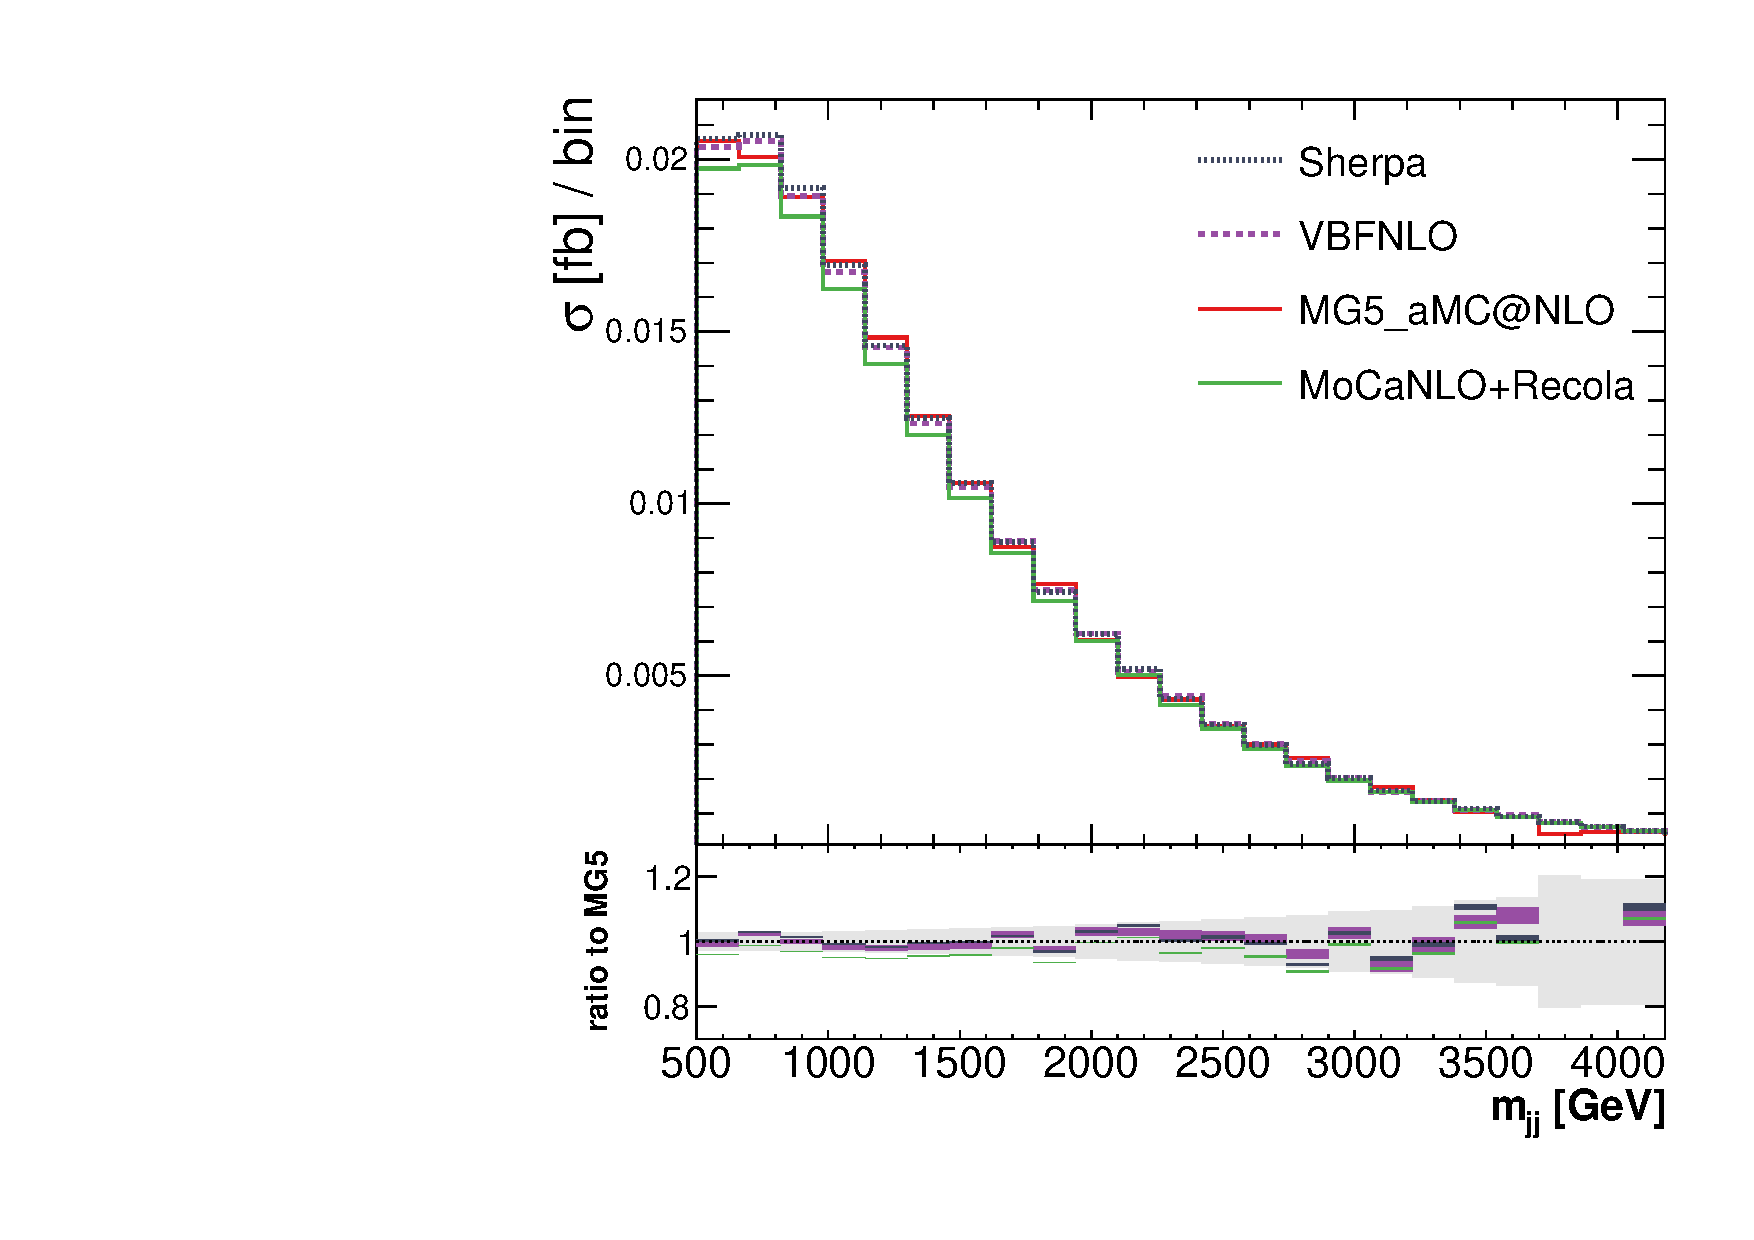
\includegraphics[scale=0.375]{figs/mjj_FixedOrder.pdf}
   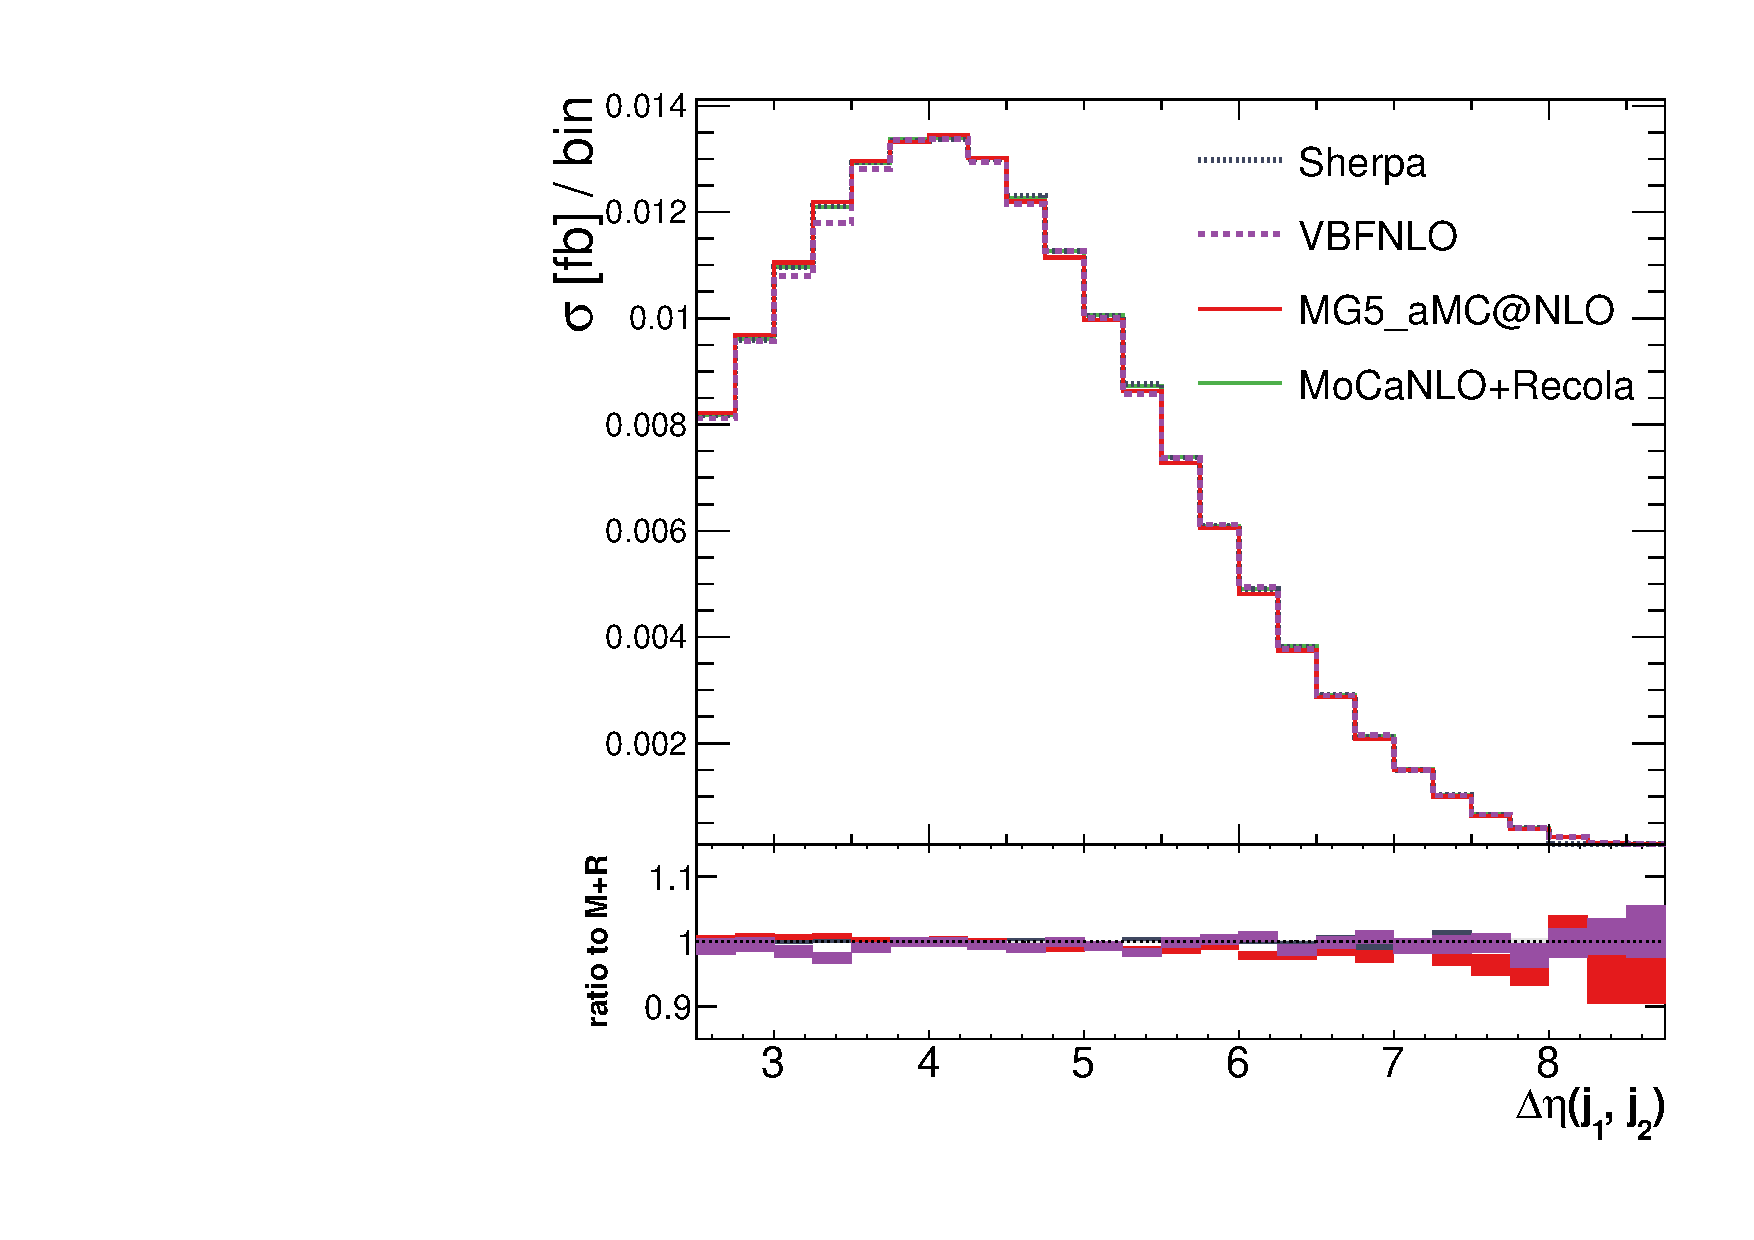
\includegraphics[scale=0.375]{figs/dEtajj_FixedOrder.pdf}
\caption{Differential distributions computed at fixed-order with centre-of-mass energy $\sqrt{s}=13{\rm~TeV}$ at the LHC for ${\rm p} {\rm p}
  \to {\rm e}^-  \nu_{\rm e}  \mu^+ \mu^- {\rm j} {\rm j}$ at LO with fixed scaled $\mu = M_{\rm W}$: 
                invariant mass of the two jets~(left),
                rapidity separation between the two jets~(right).
                The predictions in the lower plot are normalised to the ones of {\sc MG5\_aMC}. Uncertainties
                shown in the ratio plot are statistical only.
                }
\label{vbs_fig_fixed_order}
\end{center}
\end{figure}


\subsubsection*{Comparisons after parton shower}

In Figs.~\ref{vbs_fig_shower_1a} and \ref{vbs_fig_shower_1b}, a comparison of results obtained with different
generators for the process ${\rm p} {\rm p} \to {\rm e}^+  \nu_{\rm e}  \mu^+ \mu^- {\rm j} {\rm j}$ at LO supplemented with parton shower with fixed scaled $\mu =M_W$ is shown. 
In particular, in Fig.~\ref{vbs_fig_shower_1a} several differential distributions are shown:
the invariant mass of the two jets, the rapidity separation between the two jets, the transverse momentum of the anti-muon--muon system, and the distance between the two jets.
The overall picture is that the predictions obtained from {\sc Sherpa}, {\sc VBFNLO}+{\sc PYTHIA8}, and {\sc MG5\_aMC}+{\sc PYTHIA8} agree rather well over the whole kinematic range.
On the other hand, the predictions obtained from {\sc VBFNLO}+{\sc HERWIG7} seem to be very different for all type of distributions.
\MP{What is the band? Statistical error or scale uncertainty? This should be specified in the text and the caption of the plots.} 
\KL{We should decide how to present the results. Since it seems something is not right with the VBFNLO+Herwig plots (they look different
    to the VBNFLO standalone + Herwig LHE showered). Do we want to show those results instead?}
\SB{From the Sherpa side those errors are only statistical. I would guess it is the same for the rest, but please specify. For VBNFLO+Herwig: Did you check the problem with the doubled histograms I wrote in an email about? Otherwise I have no idea that's easy to check.}
\begin{figure}[htbp]
\begin{center}
   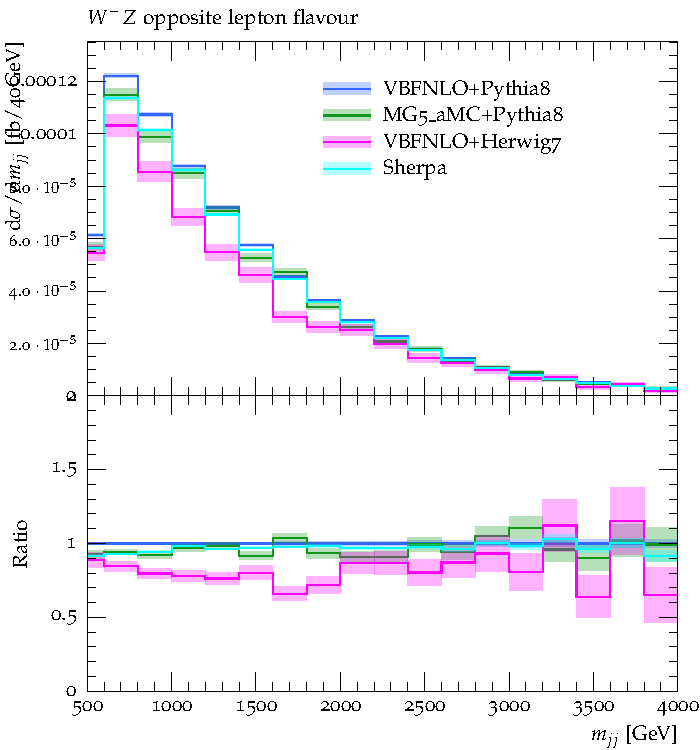
\includegraphics[scale=0.65]{figs/VBFNLO_WmZ_OF_mjj}
   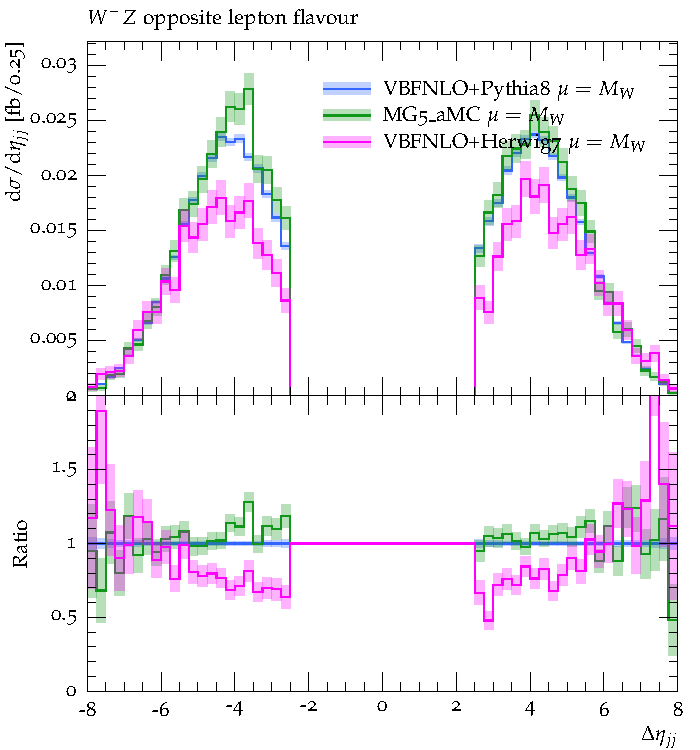
\includegraphics[scale=0.65]{figs/VBFNLO_WmZ_OF_dEtajj}
   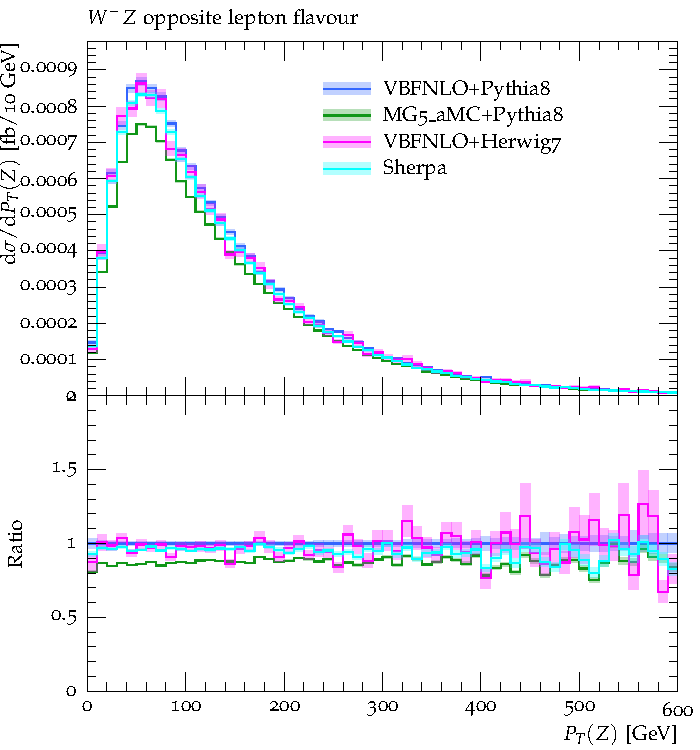
\includegraphics[scale=0.65]{figs/VBFNLO_WmZ_OF_ZPt}
   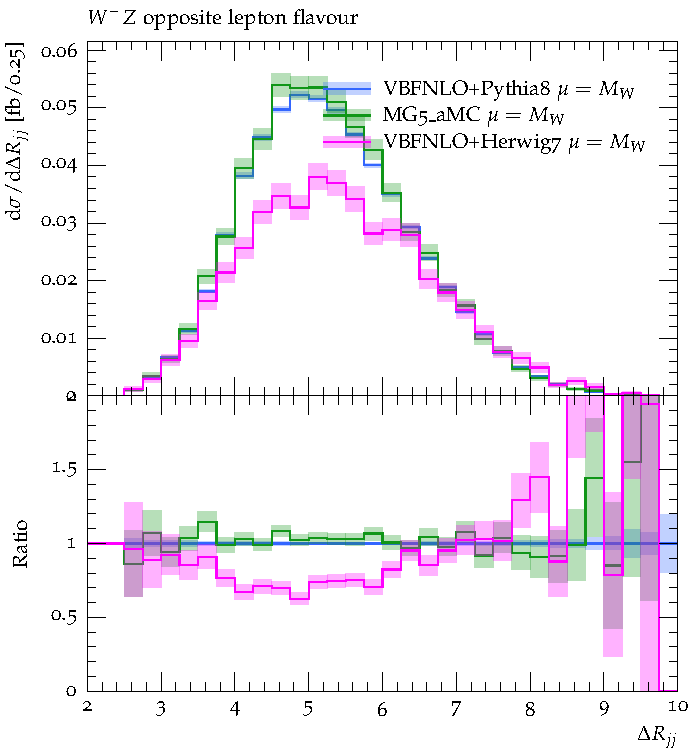
\includegraphics[scale=0.65]{figs/VBFNLO_WmZ_OF_dRjj}
\caption{Differential distributions at a centre-of-mass energy $\sqrt{s}=13{\rm TeV}$ at the LHC for ${\rm p} {\rm p}
  \to {\rm e}^-  \nu_{\rm e}  \mu^+ \mu^- {\rm j} {\rm j}$ at LO with fixed scaled $\mu = M_{\rm W}$: 
                invariant mass of the two jets~(top left),
                rapidity separation between the two jets~(top right)
                transverse momentum of the anti-muon--muon system~(bottom left), and
                distance between the two jets~(bottom right).}
\label{vbs_fig_shower_1a}
\end{center}
\end{figure}

These differences are more pronounced in Fig.~\ref{vbs_fig_shower_1b} that displays the Zeppenfeld variable for the three charged leptons and the third jet as well as the number of jets.
The Zeppenfeld variable for a given particle $X$ is defined as

\begin{equation}
  z_{X} = \frac{y_{X}-\frac{y_{{\rm j}_1}+y_{{\rm j}_2}}2}{|y_{{\rm j}_1}-y_{{\rm j}_2}|} ,
\end{equation}
%
where $y_{{\rm j}_{1/2}}$ are the rapidity of the first and second hardest jet, respectively.
The Zeppenfeld variable of the third jet, as well as the number of jets beyond two, are observables that are not defined at LO,
and are only non-zero thanks to the emissions of the parton shower.
It is thus expected that these feature an even worse agreement than the previously discussed observables, as 
significantly different algorithms are employed by the parton shower generators we consider. 
We note that even where there are similarities, we have not taken care to tune the parameters
of the shower but rather consider the spread of predictions as reflective of the uncertainty 
of the parton shower dominated observables. While variables such as the Zeppenfeld of the third jet
have known separation power between the EW and QCD induced production, tuning an experimental selection 
on this observable would introduce large theoretical uncertainties, especially if only LO predictions
are considered. A similar argument holds for a veto on extra jet activity.

\begin{figure}[htbp]
\begin{center}
   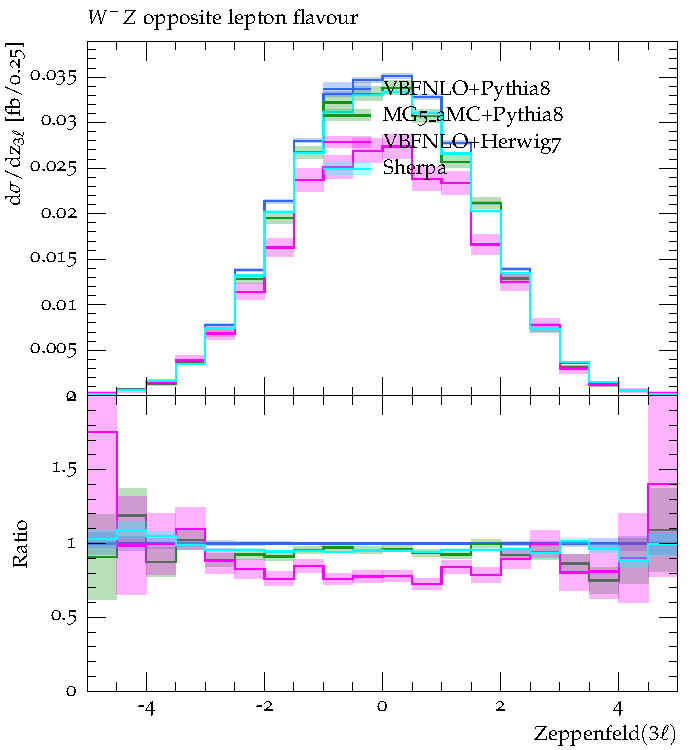
\includegraphics[scale=0.65]{figs/VBFNLO_WmZ_OF_zep3l}
   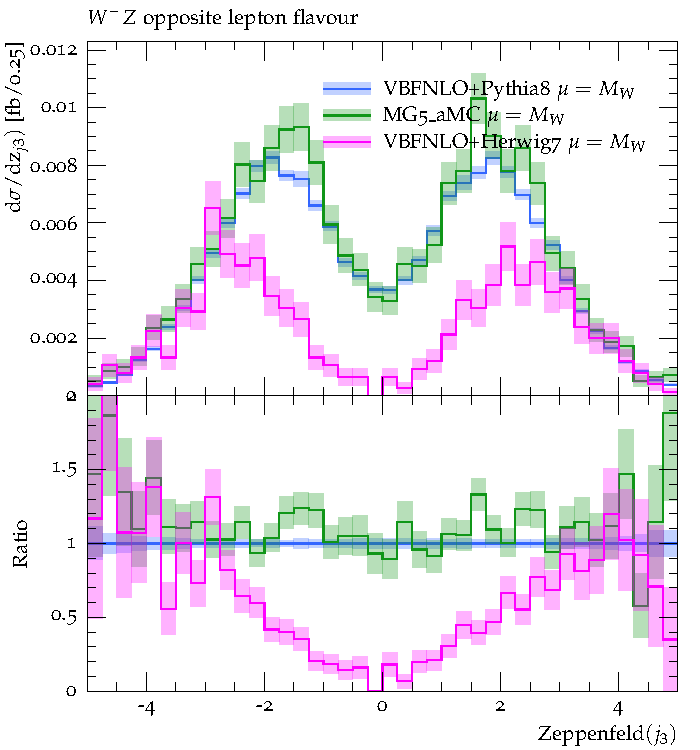
\includegraphics[scale=0.65]{figs/VBFNLO_WmZ_OF_zepj3}
   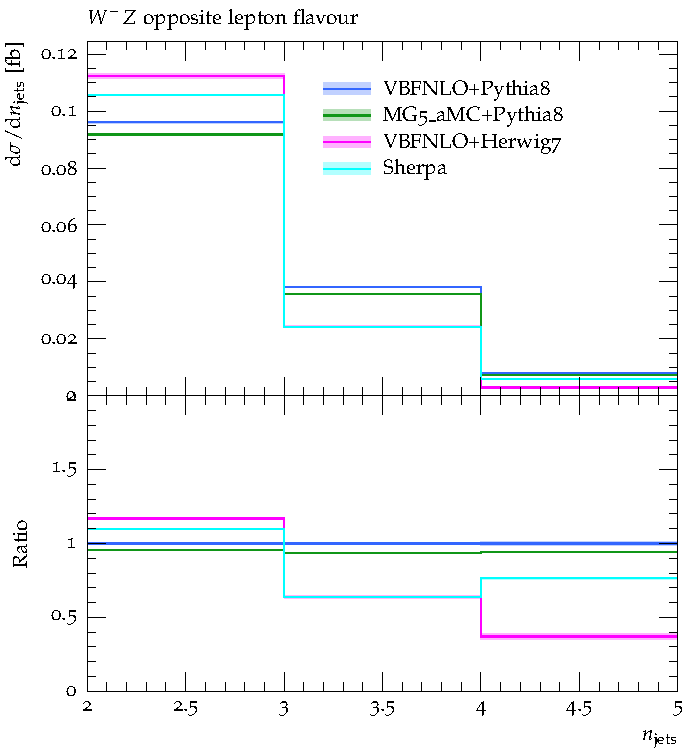
\includegraphics[scale=0.65]{figs/VBFNLO_WmZ_OF_nJets}
\caption{Differential distributions at a centre-of-mass energy $\sqrt{s}=13{\rm TeV}$ at the LHC for ${\rm p} {\rm p}
  \to {\rm e}^-  \nu_{\rm e}  \mu^+ \mu^- {\rm j} {\rm j}$ at LO with fixed scaled $\mu = M_{\rm W}$: 
                Zeppenfeld variable for the three leptons~(top left),
                Zeppenfeld variable for the third jet~(top right)
                number of jets~(bottom).
                }
\label{vbs_fig_shower_1b}
\end{center}
\end{figure}

In Figs.~\ref{vbs_fig_shower_2a} and \ref{vbs_fig_shower_2b} results obtained using the fixed scale $\mu = M_{\rm W}$ and dynamic scale $\mu = {\rm Max}\left[p_{\rm T, j}\right]$ are compared.
In particular, predictions for {\sc Sherpa} and {\sc MG5\_aMC} for both scales are presented.
The observables displayed are the same as the ones used for the previous comparison.
For the invariant mass of the two jets as well as the transverse momentum of the anti-muon--muon system, for both generators, the use of fixed scale enhance the predictions toward high transverse momentum.
For the rapidity separation of the two jets as well as the distance between the two jets, the shape difference between fixed and dynamical scale is not present for {\sc MG5\_aMC}.
On the other hand, in {\sc Sherpa}, the use of fixed scale enhances the predictions for small separations.

\begin{figure}[htbp]
\begin{center}
   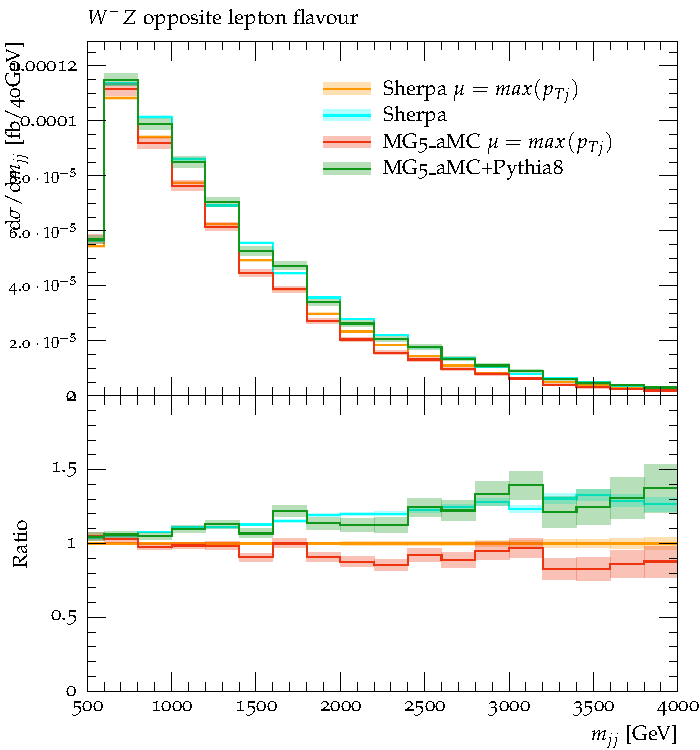
\includegraphics[scale=0.65]{figs/dyn_WmZ_OF_mjj}
   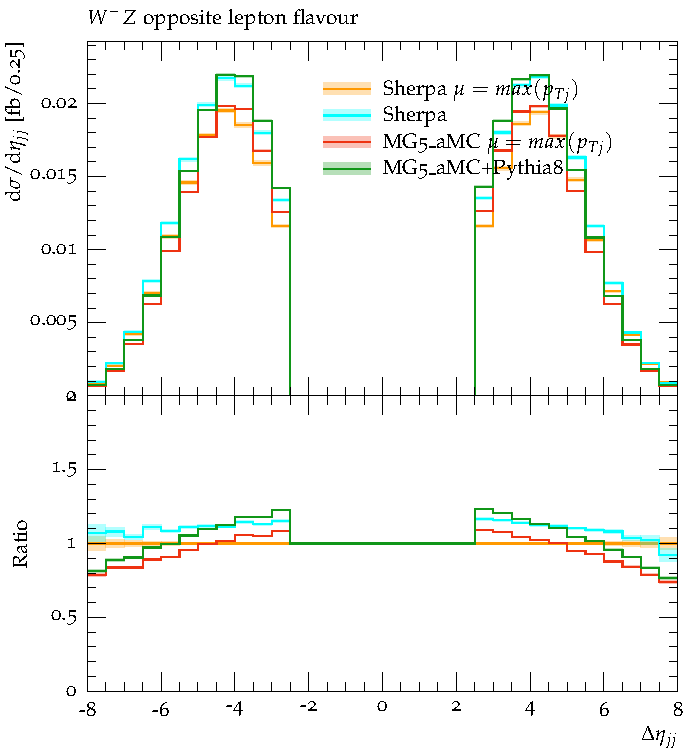
\includegraphics[scale=0.65]{figs/dyn_WmZ_OF_dEtajj}
   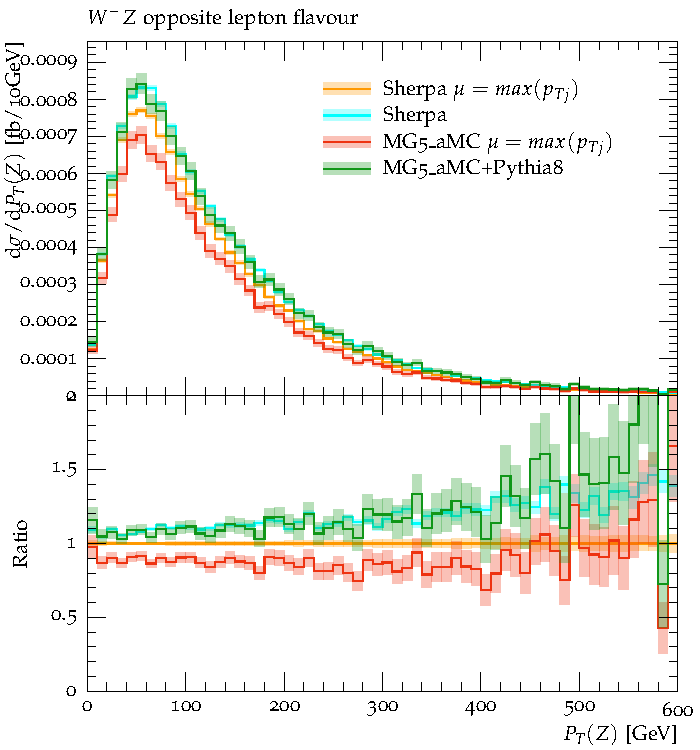
\includegraphics[scale=0.65]{figs/dyn_WmZ_OF_ZPt}
   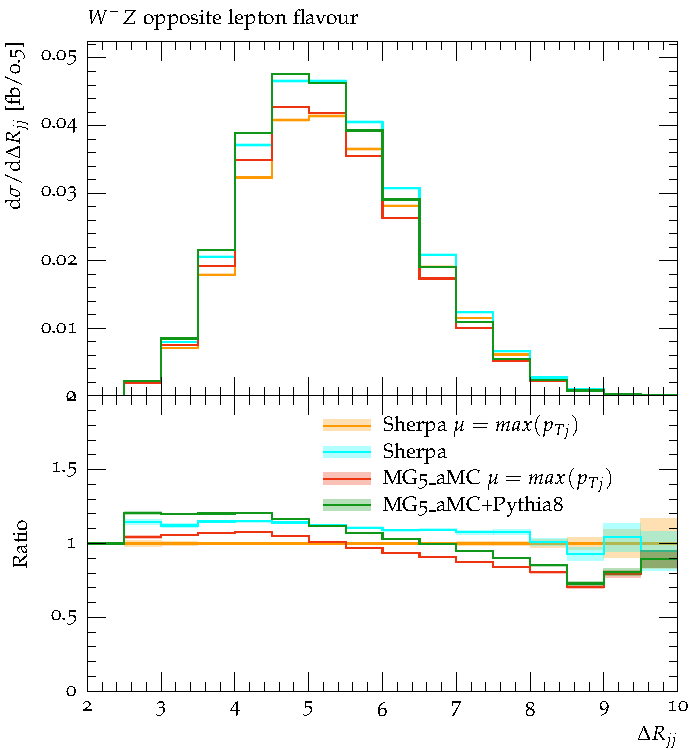
\includegraphics[scale=0.65]{figs/dyn_WmZ_OF_dRjj}
\caption{Differential distributions at a centre-of-mass energy $\sqrt{s}=13{\rm TeV}$ at the LHC for ${\rm p} {\rm p}
  \to {\rm e}^-  \nu_{\rm e}  \mu^+ \mu^- {\rm j} {\rm j}$ at LO with fixed and dynamic scale values:  
                invariant mass of the two jets~(top left),
                rapidity separation between the two jets~(top right)
                transverse momentum of the anti-muon--muon system~(bottom left), and
                distance between the two jets~(bottom right).
                In the lower plots, the predictions are normalised to the ones of {\sc Sherpa} with dynamical scale.}
\label{vbs_fig_shower_2a}
\end{center}
\end{figure}

Concerning the last set of observables (Zeppenfeld variable of the three leptons and third jet as well as the number of jets) in Fig.~\ref{vbs_fig_shower_2b}, the use of fixed or dynamical scale does not have a large impact.
The only clearly visible difference between fixed and dynamical scale is the normalisation.
This effect is already observed at the level of the fiducial cross section in Tables~\ref{table:xsectLOfix} and \ref{table:xsectLOdyn}.
The effect of the different scale amounts to a change in normalisation of about $12\%$ for both ${\rm p}{\rm p}\to{\rm e}^+\nu_{\rm e}\mu^+\mu^-{\rm j}{\rm j}$ and ${\rm p}{\rm p}\to{\rm e}^-\bar\nu_{\rm e}\mu^+\mu^-{\rm j}{\rm j}$ processes.

\begin{figure}[htbp]
\begin{center}
   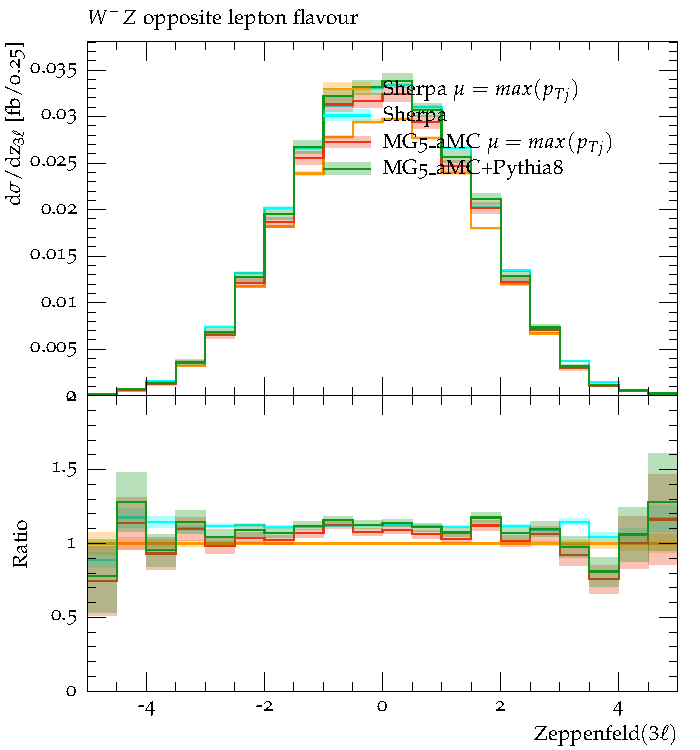
\includegraphics[scale=0.65]{figs/dyn_WmZ_OF_zep3l}
   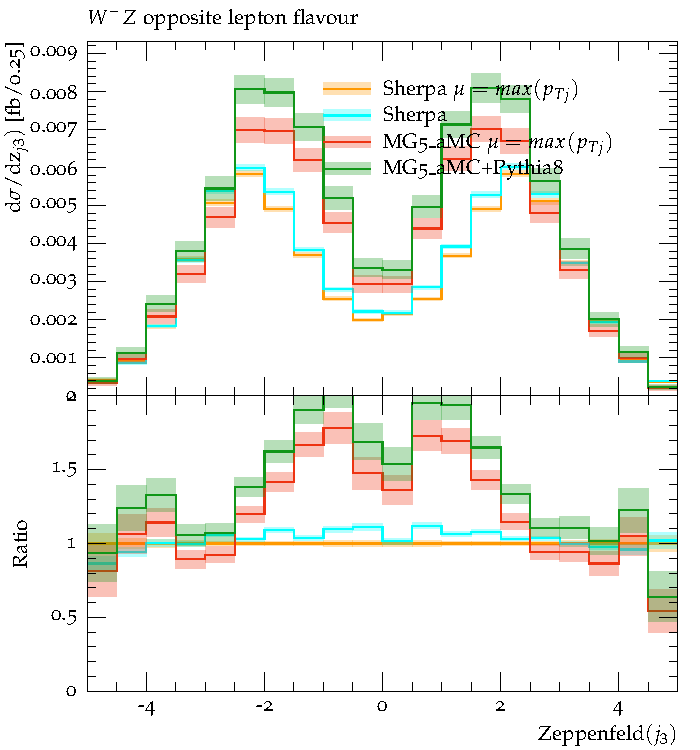
\includegraphics[scale=0.65]{figs/dyn_WmZ_OF_zepj3}
   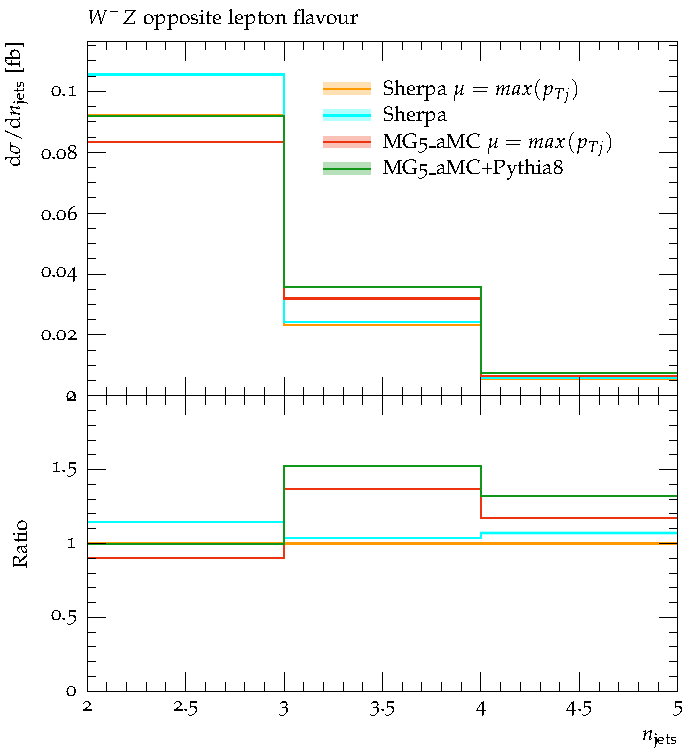
\includegraphics[scale=0.65]{figs/dyn_WmZ_OF_nJets}
\caption{Differential distributions at a centre-of-mass energy $\sqrt{s}=13{\rm TeV}$ at the LHC for ${\rm p} {\rm p} \to {\rm e}^-  \nu_{\rm e}  \mu^+ \mu^- {\rm j} {\rm j}$ at LO with fixed and dynamic scale values: 
                Zeppenfeld variable for the three leptons~(top left),
                Zeppenfeld variable for the third jet~(top right)
                number of jets~(bottom).
                In the lower plots, the predictions are normalised to the ones of {\sc Sherpa} with dynamical scale.
                }
\label{vbs_fig_shower_2b}
\end{center}
\end{figure}



\subsection{Conclusions \label{vbs_concl}}

0.2783(3)The measurement of the EW component of the ${\rm p}{\rm p} \to {\rm W}^{\pm}{\rm Z}{\rm j}{\rm j}$ process constitute a real challenge for experimental collaborations.
Such a measurement is complicated for several reasons including the low cross section and the overwhelming irreducible background.
Therefore, they have to rely on theoretical predictions in order to extract a signal.
This makes theoretical predictions implemented in various Monte Carlo programs very important.
It is thus key to have a good control over these predictions.
To that end we have performed a LO comparison of different theoretical predictions supplemented by parton shower.

Concerning the comparisons at parton level, the agreement between the various theoretical predictions is reasonable good.
This statement holds at both the level of the cross section and differential distributions.
This implies that, as for the ${\rm W}^\pm{\rm W}^\pm{\rm j}{\rm j}$ signature \cite{Anders:2018gfr}, the VBS approximation seems to be good in the typical fiducial regions used by experimental collaborations for they measurements.
In addition, the interference between the QCD and EW amplitude is also negligible.

After parton shower, the agreement is in general worse \MP{To be specified as a function of the final results/comments}.
We emphasis that this is a \emph{tuned} comparison where special care had taken to try to match all inputs of these programs.\SB{For the fixed order I agree, for the showered part I would not say that we have tuned much (at least from the Sherpa side).}

The present preliminary results.


%\clearpage
\bibliography{vbs_bib}

\end{document}
